
\section{Machine Learning Pipeline}\label{sec:machine_learning_pipeline}

In this section, we explain the machine learning pipeline that converts vacancy posting text into continuous numerical 
vectors. We leverage the structured nature of job descriptions to extract high-signal information efficiently. Job 
descriptions, despite their length, follow a consistent format. We focus on the easily detectable Mandatory and 
Desired Skills sections, which provide concentrated information about skill and competency requirements. Using the 
Spacy natural language processing library, we parse these sections to extract key technical skills such as programming 
languages (e.g., Java, Asp.Net), web frameworks (e.g., Django), and testing tools (e.g., Selenium).

While knowledge of technologies is important, the Responsibilities section conveys crucial functional aspects of the 
role. These can vary notably even between positions requiring similar technology skills, such as developers, testers, 
and support engineers. The section typically lists tasks to be performed, which might include 'develop big data strategy,' 
'conduct code reviews,' 'engage with stakeholders' or 'application development.' We extract such task descriptions from 
job responsibilities by employing natural language processing techniques. This includes part-of-speech tagging to identify 
action verbs and dependency parsing to locate their direct objects, which are then combined to form concise verb-object 
phrases representing key tasks. By leveraging the structured format and our knowledge of the postings, we effectively 
eliminate low-signal words in the description. In the following subsections, we describe our machine learning pipeline 
which adheres to two key ideas: leveraging capabilities of a pre-trained language model and utilizing past selection 
decisions. 

\subsection{Pre-trained Embeddings}

Here we describe the approach to mapping the extracted text to the embedding space of a pre-trained language model. 
To create vector representations of the two parts we employ Sentence-BERT (SBERT), a modification of the pre-trained 
BERT network \citep{devlin2018bert}. SBERT is designed to derive semantically meaningful sentence embeddings, making 
it more efficient for comparing longer text strings than BERT embeddings, which are typically word vectors, although 
the BERT word-level embeddings vary with the context, unlike their predecessors \citep{reimers-2019-sentence-bert}. 
SBERT converts text into dense vector representations, effectively capturing the semantic meanings and relationships 
between words. This model is particularly suitable for our needs because it is pre-trained and fine-tuned for 
similarity tasks, ensuring that it can generate fixed-size embeddings that are both informative and consistent. 
The embeddings are generated using the SentenceTransformers library (model: paraphrase-MiniLM-L6-v2). By leveraging 
SBERT, we ensure that our embeddings capture the nuanced language used in job descriptions, which is critical for 
accurately representing the skills and tasks. 

For every $j_i$, we have the set of words $j_i^s$ (skills) and $j_i^t$ (tasks) and obtain SBERT embeddings 
$e_i^s$ ($384 \times 1$) and $e_i^t$ ($384 \times 1$) respectively. This separation allows for more granular 
embeddings and a focused semantic representation of each aspect. These embeddings encapsulate the semantic content 
of the job descriptions, allowing us to compare and analyze them effectively. The dual-embedding approach provides 
a comprehensive view of each position, highlighting both the required competencies and the associated responsibilities. 
This detailed representation forms the foundation for developing a robust distance metric that can accurately reflect 
the similarity between job descriptions, ultimately aiding in the assessment of internal mobility and selection probabilities.  

\subsection{Dimension Reduction}

To manage the high-dimensional embeddings generated for job descriptions, we apply Principal Component Analysis (PCA) 
to reduce the dimensionality of both \(\{e_i^s\}\) and \(\{e_i^t\}\). PCA is a technique that transforms the original 
high-dimensional data into a new coordinate system with fewer dimensions while retaining most of the original variance. 
For our embeddings, we apply PCA separately to the skill embeddings \(\{e_i^s\}\) and the task embeddings \(\{e_i^t\}\), 
retaining 90\% of the variance in each case. This process reduces the skill embeddings from 384 dimensions to 49 dimensions, 
now denoted as \(\{p_i^s\}\), and the task embeddings from 384 dimensions to 124 dimensions, now denoted as \(\{p_i^t\}\).
 Notably, the dimensionality of the skills embedding (\(\dim(p_i^s) = 49\)) is smaller than that of the tasks 
 embedding (\(\dim(p_i^t) = 124\)). This indicates that a relatively small number of components capture most of 
 the information in the skills embedding, which is expected since skills are described using a more specific vocabulary 
 compared to tasks. If we concatenate the \(\{p_i^t\}\) and \(\{p_i^s\}\) embeddings, the resulting representation is 
 still 173 dimensions, which is too high for measuring a useful distance between job postings.


To further reduce the dimensionality of our job description embeddings, we perform dimension reduction via clustering. 
The core idea is to represent each of our original embeddings in terms of its membership probabilities with respect to 
cluster centers. Specifically, we calculate the membership probability of a job description for each cluster, resulting 
in a set of \(k\) probabilities for each embedding. These \(k\) probabilities form a new vector of dimension \(k\), 
effectively reducing the original high-dimensional embeddings to a more manageable size.

We employ the Fuzzy C-Means (FCM) algorithm, which allows each embedding to belong to multiple clusters with varying 
degrees of membership. The membership probabilities are values between 0 and 1 and sum to 1, forming a probabilistic 
distribution. In our implementation, we apply FCM to both the skill embeddings \(\{p_i^s\}\) and the task embeddings 
\(\{p_i^t\}\). Let \(k_s\) be the number of skill clusters and \(k_t\) be the number of task clusters. For each job 
description, FCM generates a membership probability vector \(m_i^s\) (\(k_s \times 1\)) for skills 
and \(m_i^t\) (\(k_t \times 1\)) for tasks, indicating the degree to which each job description belongs to each cluster.

Concatenating these membership probability vectors \(m_i^t\) and \(m_i^s\) results in \(x_i\), a low-dimensional 
representation of \(j_i\). This combined vector \(x_i (k * 1)\) effectively captures the key information in \(j_i\) 
while reducing the dimensionality of the data, facilitating the development of a robust distance metric tailored to 
our specific context. This lower-dimensional representation improves the accuracy and effectiveness of our internal 
mobility predictions by preserving the most relevant information for measuring distances between job postings. The 
vectorization process described is illustratively summarized in \autoref{fig:job-vectorization}. This leaves us with 
the question of selecting the number of skill and task clusters, which we will take up after we discuss the measuring 
of distances between job postings and their informativeness regarding selection probabilities to vacancies. 


\begin{figure}[htbp]
    \centering
    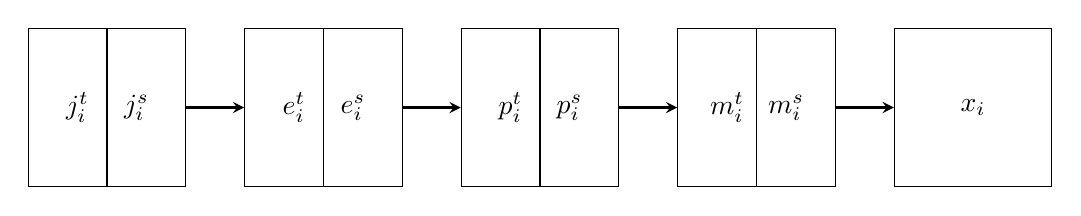
\begin{tikzpicture}
        % Styles for the squares and arrows
        \tikzset{
            square/.style={
                draw,
                rectangle,
                minimum size= 2cm,
                fill=none,
                align=center
            },
            arrow/.style={
                thick,
                ->,
                >=stealth 
            }
        } 
        % Define initial position and shift for squares
        \def\initpos{0}
        \def\shift{2.75}  % Distance between centers of squares
        % Custom labels for each step in the process
        \def\labelsT{{"j_i^t", "e_i^t", "p_i^t", "m_i^t"}}
        \def\labelsS{{"j_i^s", "e_i^s", "p_i^s", "m_i^s"}}
        % Drawing the squares, split squares, and arrows
        \foreach \i in {0,...,4} {
            % Draw split square for the first four
            \ifnum\i<4
                \node[square] (square\i) at (\initpos+\shift*\i,0) {};
                \draw (square\i.south) -- (square\i.north);
                \node at ([xshift=-0.375cm] square\i.center) {$\pgfmathparse{\labelsT[\i]}\pgfmathresult$};
                \node at ([xshift=0.375cm] square\i.center) {$\pgfmathparse{\labelsS[\i]}\pgfmathresult$};
            \else
                % Draw the unsplit square for the fifth one
                \node[square] (square\i) at (\initpos+\shift*\i,0) {$x_i$};
            \fi
            % Draw arrow to next square
            \ifnum\i>0
                \draw[arrow] (square\the\numexpr\i-1\relax.east) -- (square\i.west);
            \fi
        }
    \end{tikzpicture}
    
    \vspace{1em}
    
    \begin{center}
        \small
        \begin{tabular}{lll}
            \textbf{Notation} & \textbf{Description} & \textbf{Dimensions} \\
            \hline
            $j_i^{t/s}$ & Split to task and skill components of $j_i$ & text \\
            $e_i^{t/s}$ & $\text{SBERT}(j_i^{t/s})$ & $384 \times 1$ \\
            $p_i^{t/s}$ & $\text{PCA}(e_i^{t/s})$  & $124 \times 1$ (tasks), $49 \times 1$ (skills) \\
            $m_i^{t/s}$ & $\text{FuzzyC}(p_i^{t/s})$  & $k_t \times 1$ , $k_s \times 1$  \\
            $x_i$ & $m_i^t \oplus m_i^s$ & $k_t + k_s \times 1$ \\
        \end{tabular}
    \end{center}
    
    \caption{This is a pictorial representation of the vectorization process that captures the information in a job posting to a numerical vector. The table provides a summary of the notation and dimensions used at each step of the process.}
    \label{fig:job-vectorization}
\end{figure}



\subsection{Distance Metric Learning} 

Now that we have represented the textual job descriptions in a vector format, we test whether these representations capture 
meaningful skill information by learning a distance metric that predicts selection outcomes. In formulating this distance, 
our two major ideas included leveraging the capabilities of pre-trained language models and using past selection decisions 
in a supervisory capacity to learn which aspects of posting content are most informative for predicting selection.

The ability to learn a custom metric is advantageous because it allows us to create a distance function tailored to the 
specific characteristics and selection patterns of our organization. Traditional distance metrics, such as Euclidean 
distance, treat all dimensions equally and do not take into account the nuances of job descriptions and the importance 
of different skills and responsibilities in the selection process. By learning a custom distance metric, we can weigh 
the various components of \(x_i\) according to their relevance in the actual hiring decisions. For instance, if a vacancy 
requires expertise in Mainframe development but also involves some tasks related to preparing reports and using 
presentation software, the lack of expertise in Mainframe development would significantly reduce the chances of 
being selected, whereas the latter skills, which are easier to acquire, would have less impact. This approach leads 
to a more accurate and informative measure of job similarity. In other words, our goal is to craft a distance that is 
specifically adapted to the problem of assessing skill adequacy for filling the vacancy.

We will focus on learning a distance from the family of Mahalanobis distances, which are parameterized by a 
matrix \(M\). The core idea is that dimensions contributing less to the distance should receive lower weight. 
For example, if a vacancy requires expertise in Mainframe development but only some competence in word processing, 
the latter skill will be weighted less in the distance measure. If the matrix is diagonal, the distance calculation 
represents a stretch for each dimension. Irrelevant covariates will be compressed so that their values are always 
effectively zero. Highly relevant covariates will be stretched so that for two units to be considered a match, 
they must have very similar values for those covariates. In this way, diagonal matrices lead to very interpretable 
distance metrics. If the Mahalanobis distance matrix is not constrained to be diagonal, then it induces a stretch 
and rotation, leading to more flexible albeit less interpretable notions of distance. The distance function we aim 
to learn is defined as:

\begin{equation}
d(x_v, x_c; M) = \sqrt{(x_v - x_c)^T M (x_v - x_c)}
\end{equation}
Here, \(x_v\) and \(x_c\) are the vector representations of the competencies required at the sought vacancy \(v\) and 
the current job \(c\), respectively and $M$ is a positive semi-definite matrix.

Our dataset \(A\) consists of tuples \((x_v, x_c, S_{v,c})\), where \(j_v\) is the current job description, \(j_c\) is 
the sought vacancy description, and \(S_{v,c}\) is the binary selection indicator. Our focus is on a distance that can 
discriminate between skill distances in the set of \textit{plausible} applications, whose empirical counterpart is \(A\). 
In other words, we want \(M\) such that the distance between cases that resulted in rejection is larger compared to cases 
that resulted in selection. We utilize the past selection and rejection data to inform our metric learning process. 
Specifically, we adopt the Mahalanobis Metric for Clustering (MMC) algorithm by \citep{Xing2002} to learn a distance 
function that can effectively differentiate between selected and non-selected candidates. The optimization problem solved 
is the following: 

\begin{align*}
\text{Maximize:} \quad & \sum_{(v,c): S_{v,c} = 0} d(x_v, x_c; M) \\[1em]
\text{Subject to:} \quad & \sum_{(v,c): S_{v,c} = 1} d(x_v, x_c; M)^2 \leq 1 \\
& M \succeq 0
\end{align*}


Adapting to our context, we are maximizing the sum of distances for cases that did not result in selection. The constraints 
are regularity constraints that ensure the data is not collapsed to a point and the distance satisfies the triangle 
inequality. This approach allows us to craft a distance metric \(d(x_v, x_c)\) that effectively captures the skill and 
competency fit between positions, utilizing the historical selection data to guide the learning process. Our dataset \(S\) 
comprises 1060 observations, which forms 75\% of our total data points on selection decisions. The implementation of this 
approach uses Python 3.5, with the MMC algorithm available in the sci-kit learn library, requiring no special computing 
resources. In the following subsection, we will discuss the parameter tuning process for determining the optimal length of 
embeddings, which in turn will define the size of the matrix \(M\).




\subsection{Parameter Tuning} 

To implement the algorithm, we need to determine the optimal number of clusters ($k_t$, $k_s$) for the reduced task and 
skill embeddings, which will define the final representation $x_i$ of a job description. This selection must be data-driven 
to ensure the most accurate distance metric for predicting selection probabilities. Using our dataset of 1,370 internal a
pplications and their outcomes (excluding rejections in favor of other internal applicants), we employ 5-fold cross-validation 
on the application dataset $A$. We iteratively test combinations of $k_s$ and $k_t$, where $k_s, k_t \in \{2, 3, ..., 20\}$, 
subject to the constraint $k_s + k_t < 25$. This constraint is a practical one: with limited training data, we cannot allow 
the dimensionality of M to grow too large, as this could lead to overfitting. For each combination, we compute the average 
Area Under the Receiver Operating Characteristic Curve (AUC).

The results, reported in Figure \ref{fig:AUC}, show that the best model achieves an AUC of 0.62 with $k = 20$, where 
$k_s = 17$ (skill clusters) and $k_t = 3$ (task clusters). This cross-validation process ensures that the chosen number 
of clusters provides a representation that effectively captures the underlying patterns in the data, leading to a more 
accurate and informative distance metric for predicting internal mobility and selection outcomes.  

\begin{figure}[htb]
    \centering
    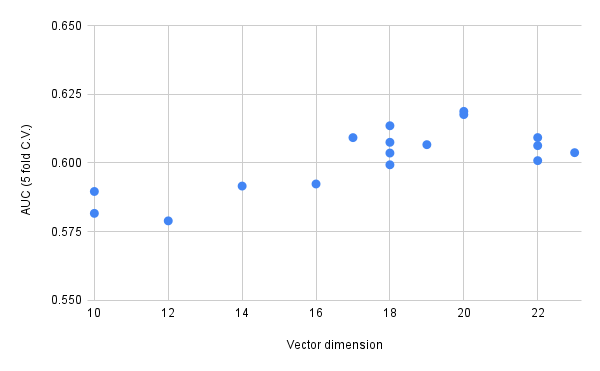
\includegraphics[width=0.75\textwidth]{new_img/chart.png}
    \caption{5 fold AUCs computed at different dimensionality of $k$}
    \label{fig:AUC}
\end{figure}


The AUC of 0.62 indicates that skill distances derived purely from job posting text have meaningful predictive power - 
the probability that a randomly chosen selected application will be ranked as better fit than a randomly chosen rejected 
application is substantially higher than chance. This demonstrates that job postings contain real information about position 
requirements that predicts selection outcomes. As we show in subsequent sections, this validation of posting informativeness 
opens new possibilities for understanding skill requirements and worker-job fit.

To recap, we developed a machine learning pipeline to test whether job posting content meaningfully captures differences in 
position requirements by predicting selection outcomes. Our approach leverages the capabilities of pre-trained language models
and the opportunity to take a supervised approach by utilizing past selection decisions. This combination of rich text 
representations and actual selection outcomes demonstrates that postings contain meaningful information about skills and 
requirements, providing a foundation for deeper analysis of how workers and firms navigate evolving skill demands.

